
\input{"C:/Users/spileggi/Google Drive/STAT 330/Lectures/SlideStyle.tex"}



\title[Lecture 4]{DATA Step Basics}
\author[Pileggi]{Shannon Pileggi}

\institute[STAT 330]{STAT 330}

\date{}


\begin{document}

\begin{frame}
\titlepage
\end{frame}

\begin{frame}
\frametitle{OUTLINE\qquad\qquad\qquad} \tableofcontents[hideallsubsections]
\end{frame}


%===========================================================================================================================
\section[Creating variables]{Creating variables}
%===========================================================================================================================
\subsection{}
\begin{frame}[fragile]
\ft{Working data set}
\bmp{0.6\textwidth}
\begin{code}{.}
DATA grades;
   INPUT name $ exam1 exam2 exam3;
   DATALINES;
   Shannon      96    82    83
   Lex          92    81    68
   Becky        92    75    73
   Lora         94    65    70
   Susan        91    77    85
   Hunter       76    72    86
   Ulric        98    71    80
   Richann      90    60    60
   Tim          97    94   100
   Ronald        .    77    60
   ;
RUN;
\end{code}
\emp
\end{frame}

\begin{frame}
\ft{Creating Variables}
\bi
\item To create a variable, use an assignment statement like
\item[] \fbox{\ttt{newvar = } \emph{expression} ; }
\item The left hand of the equal sign is the variable name, the right hand of the expression may be a constant, another variable, or an expression
\item The variable type (numeric or character) is determined by the expression that defines it.
\item When creating numeric variables, SAS follows standard order of operations (PEMDAS = parentheses, exponents, multiplication/division, addition/subtraction)
\ei
\end{frame}

\begin{frame}[fragile]
\ft{Creating variables, part 1}
\hspace*{-0.2in}\bmp{0.43\textwidth}
\begin{code}{.}
DATA grades2 ;
  SET grades;
  sec_num = 70 ;
  sec_char = "70" ;
  exam1_new = exam1;
  miss_num = . ;
  miss_char = " " ;
RUN ;
\end{code}
\emp
\bmp{0.02\textwidth} \hspace{0.1in} \emp
\bmp{0.60\textwidth}
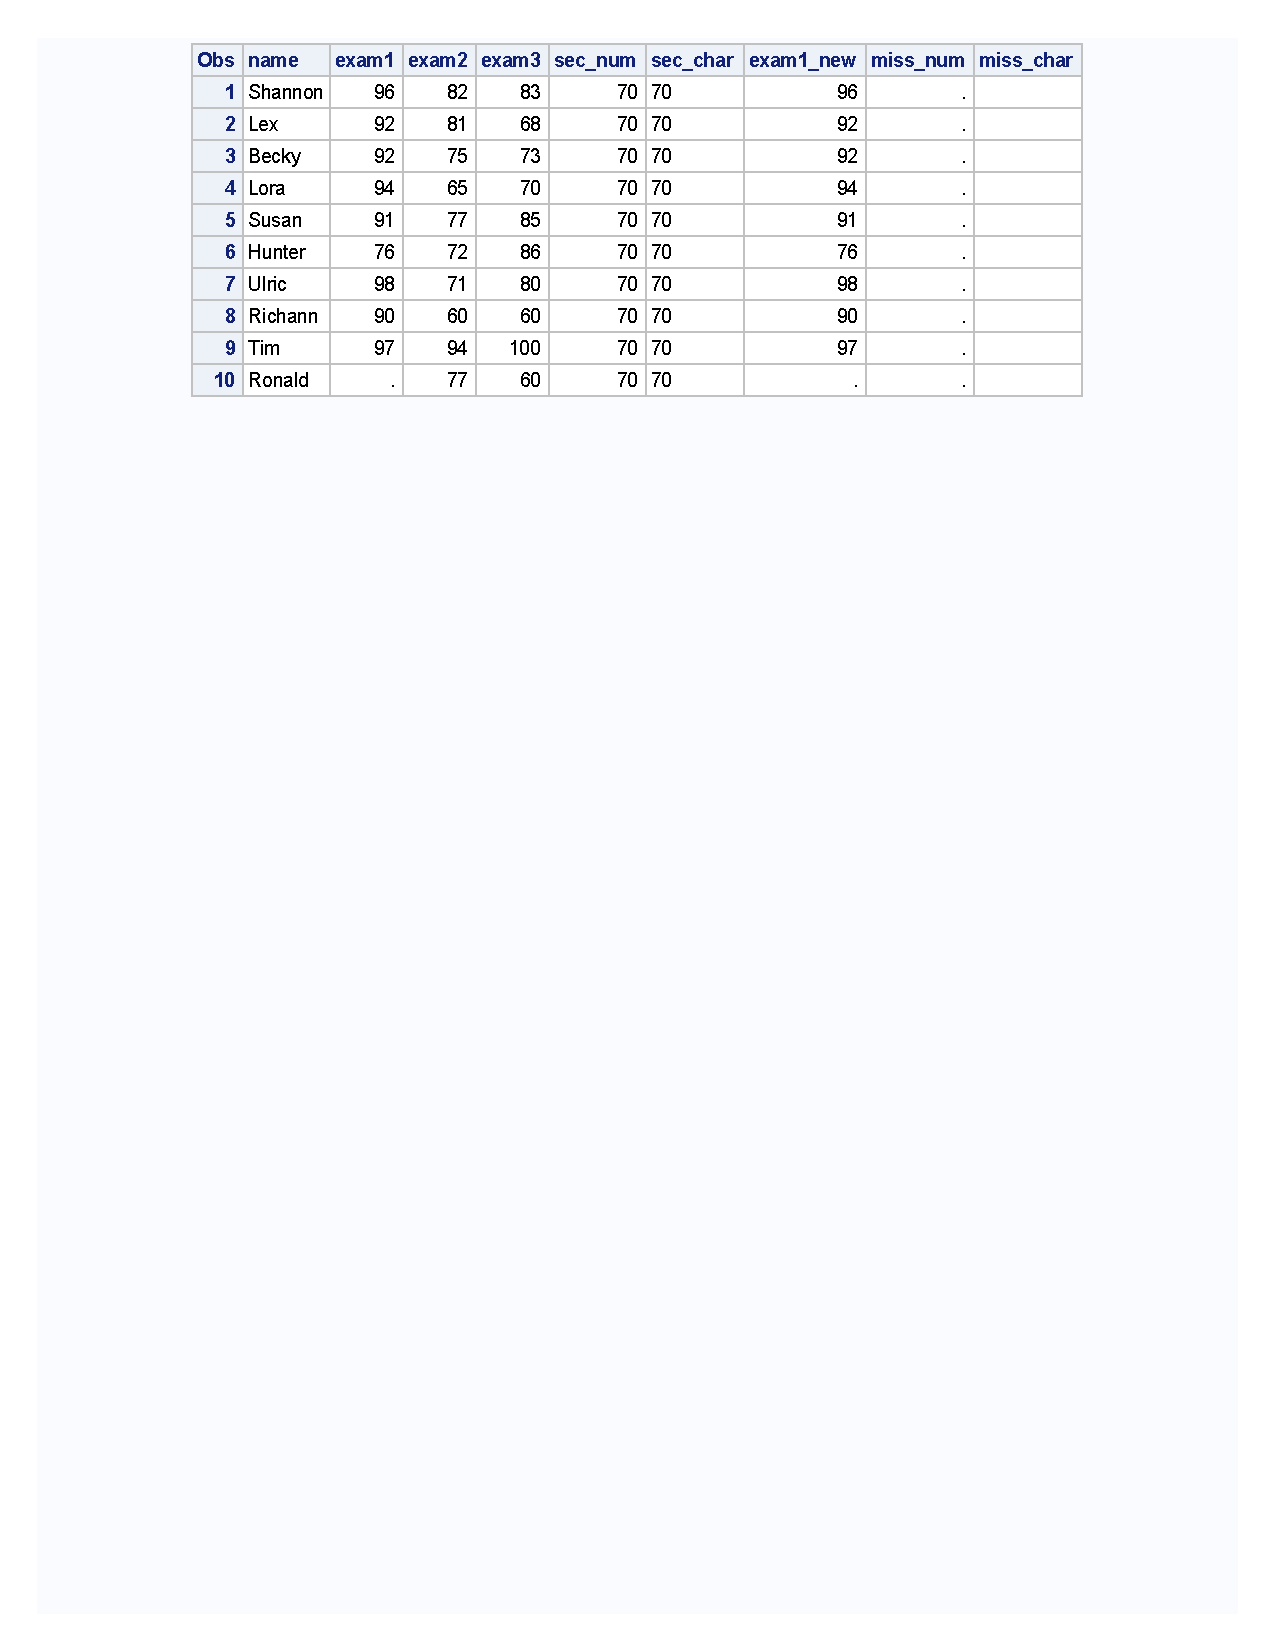
\includegraphics[trim=3cm 21cm 3cm 0.5cm,clip,width=1.0\textwidth]{L5_newvars.pdf}
\emp\\
\bi
\item[]
\item character values go in quotations
\item \ttt{sec\_num, sec\_char} are assigned \emph{constant} values
\item \ttt{miss\_num, miss\_char} are assigned missing values
\item \ttt{exam1\_new} is assigned the value of another variable
\ei
\end{frame}

\begin{frame}[fragile]
\ft{Creating variables, part 2}
\bmp{0.85\textwidth}
\begin{code}{.}
DATA grades2 ;
   SET grades;
   ave_exam1 = (exam1 + exam2 + exam3)/3 ;
   ave_exam2 =  MEAN(exam1, exam2, exam3) ;
RUN ;
\end{code}
\emp\\
%\bmp{0.45\textwidth}
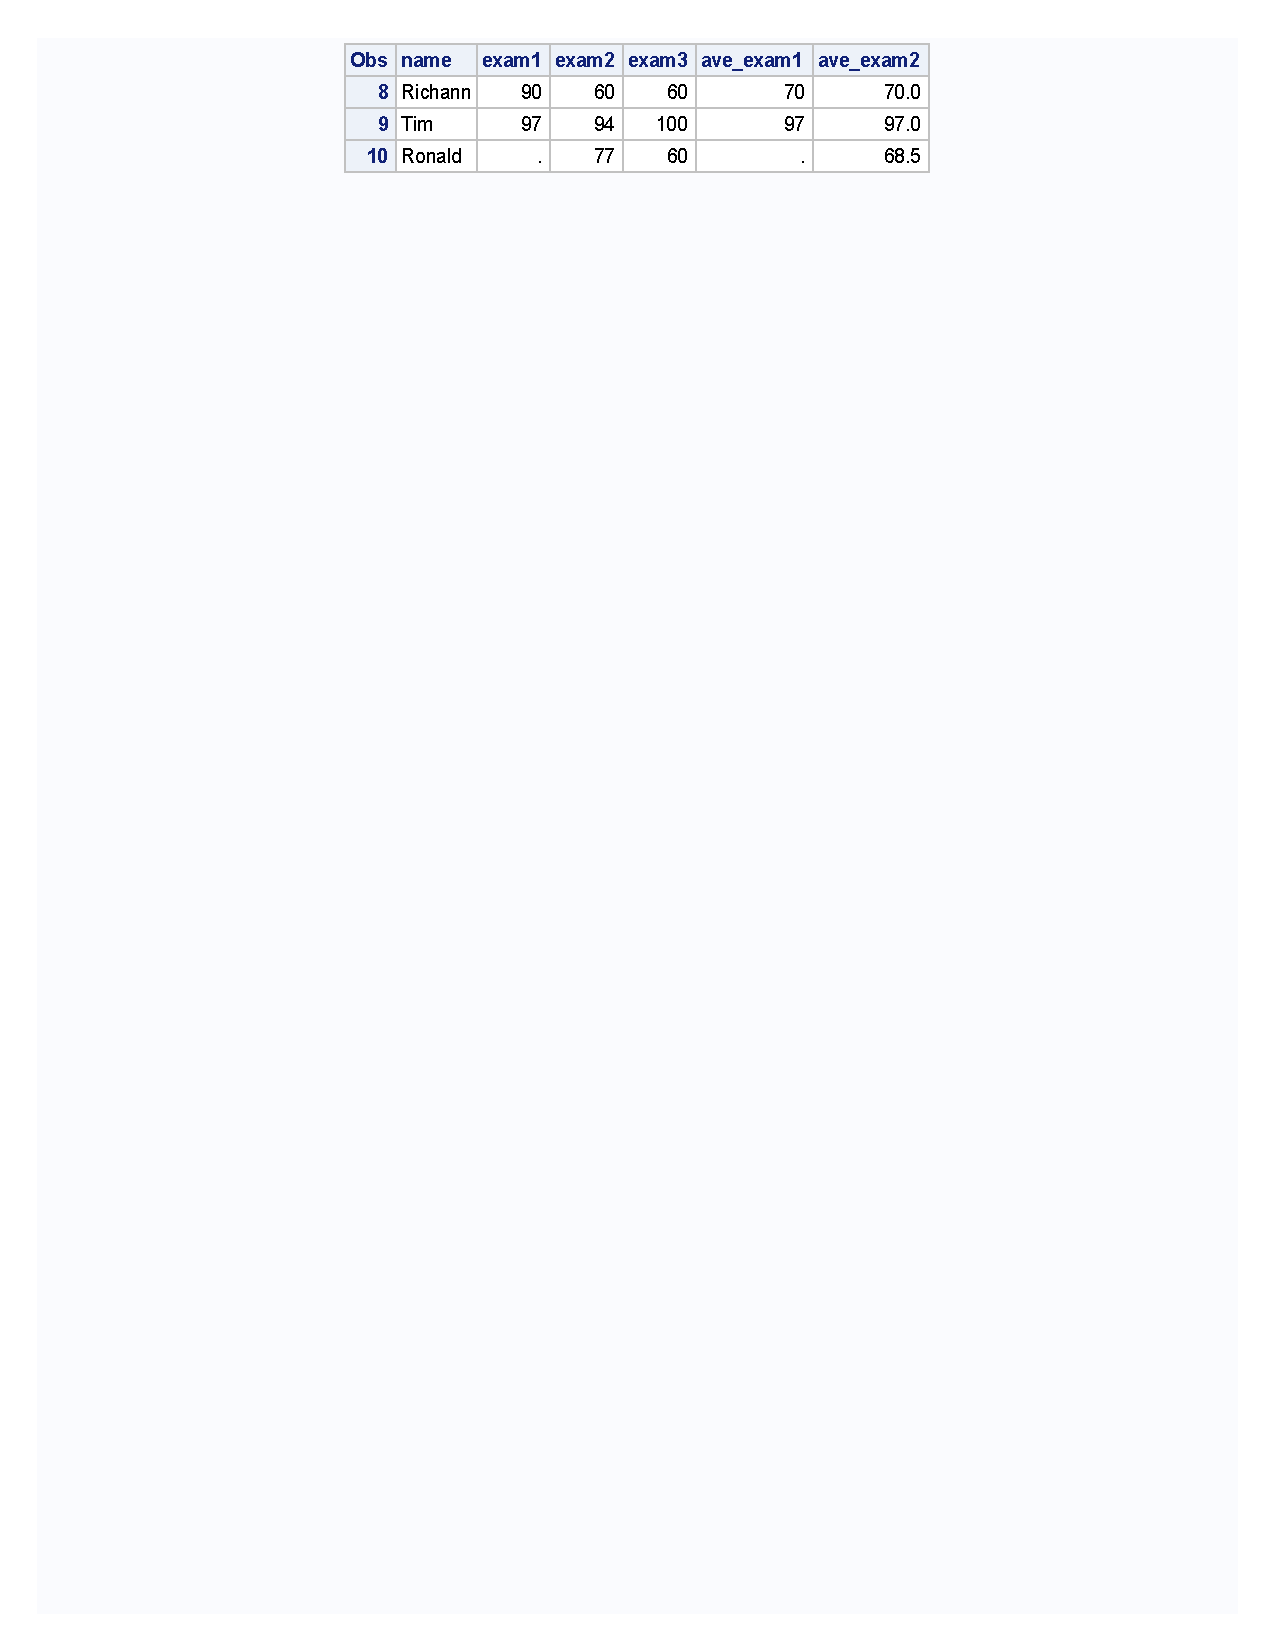
\includegraphics[trim={5cm 25cm 5cm 0.5cm},clip,width=0.7\textwidth]{L4_means.pdf}
\bi
\item \ttt{ave\_exam1} is calculated by an expression
\item[] expressions can result in \emph{propagation of missing values}
%\item[]
\item \ttt{ave\_exam2} is calculated by a function
\item[] functions generally operate on all non-missing values
\ei
%\emp
\end{frame}


\begin{frame}
\ft{SAS functions}
\bi
\item Built in SAS functions allows you to simplify programming
\item SAS has nearly 300 different functions dealing with mathematical expressions, characters, dates, etc.
\item p. 78-80 of your textbook has some of the more commonly used functions
\item Functions perform operations on arguments
\bi
\item all functions require parentheses
\item functions can be nested within each other
\ei
\ei
\end{frame}

\begin{frame}[fragile]
\ft{Function practice}
\bmp{0.55\textwidth}
\begin{code}{.}
DATA grades2 ;
   SET grades ;
   first_letter = \textcolor{OrangeRed}{function()} ;
RUN ;
\end{code}
\emp
\bmp{0.05\textwidth}\hspace{1in}\emp
\bmp{0.45\textwidth}
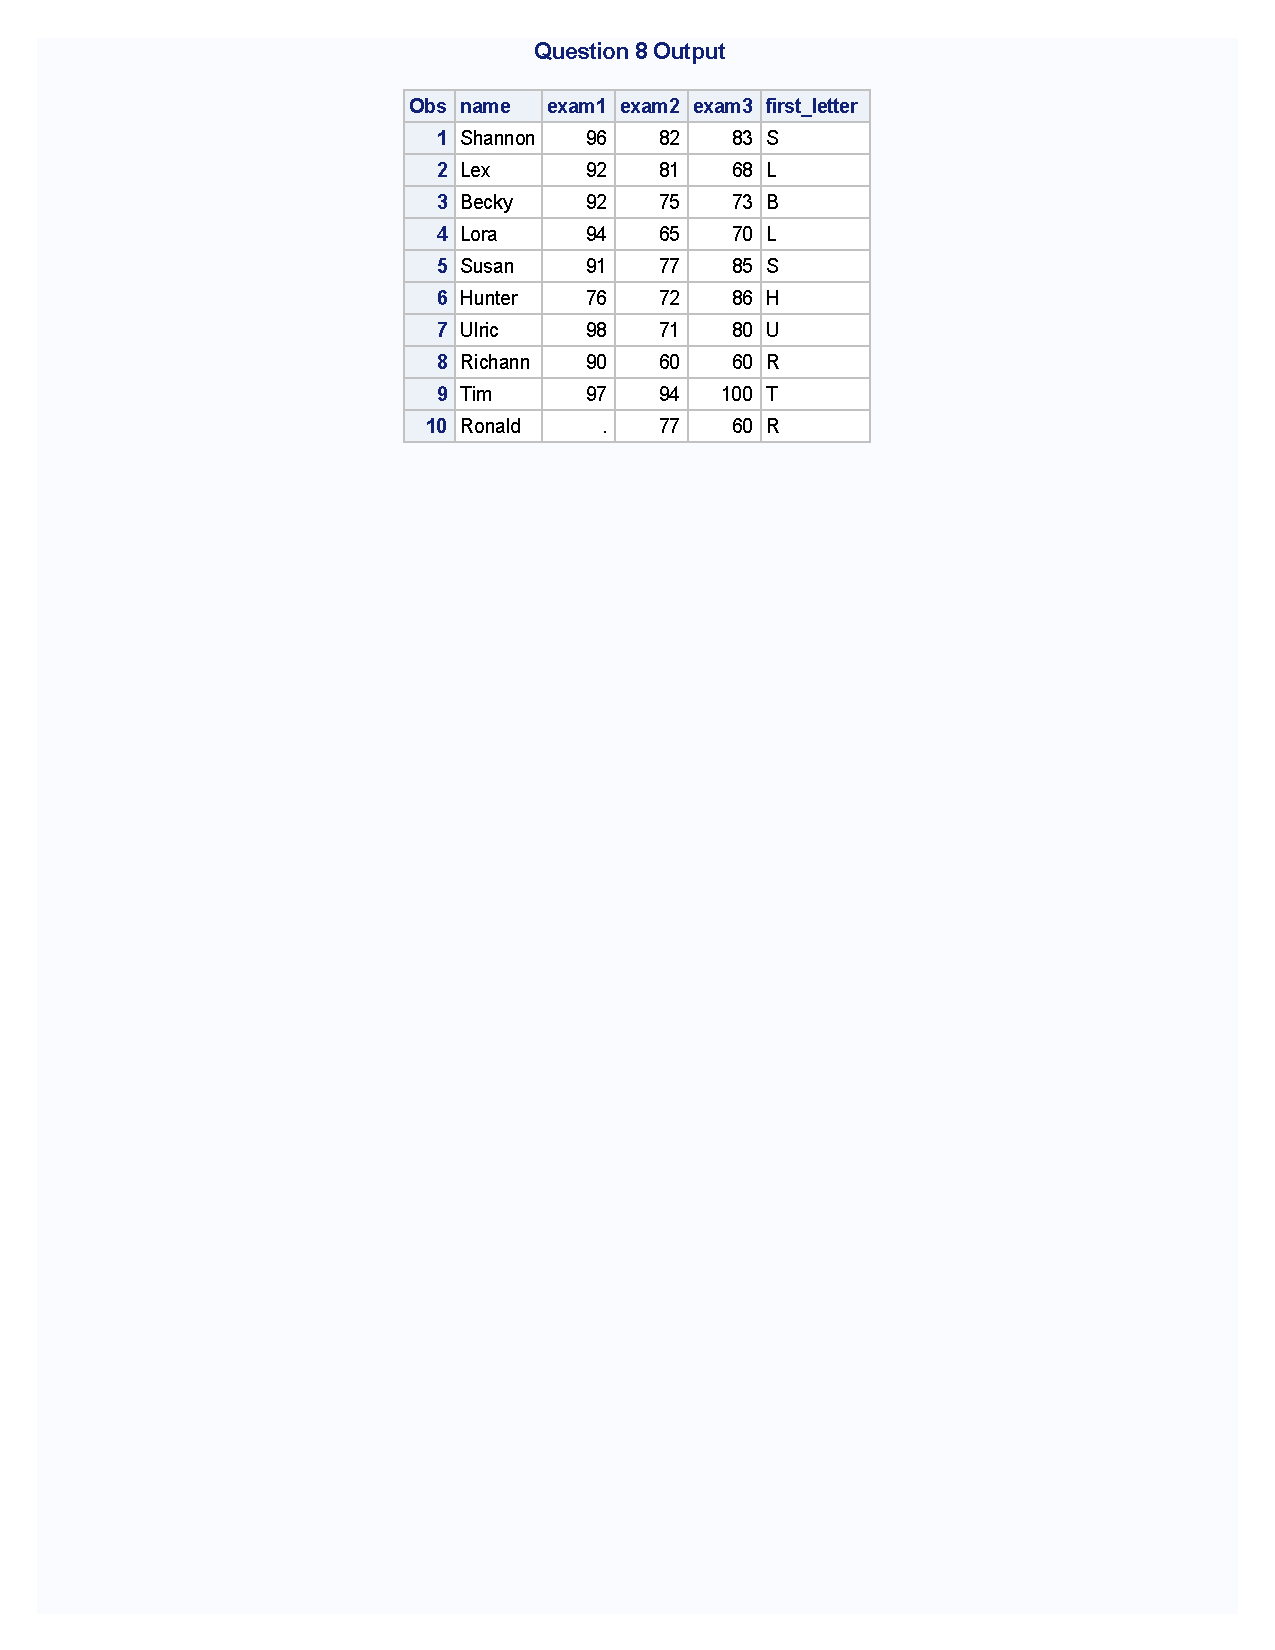
\includegraphics[trim={6cm 20cm 6cm 1.5cm},clip,width=1.0\textwidth]{L4_firstletter.pdf}
\emp\\
% first_letter = SUBSTR(name, 1, 1) ;	
\vskip10pt
\oyo
\bi
\item Search for ``SAS functions''
\item Identify a function that will allow you to extract part of a character string
\item Use this function to create a variable that represents the first letter of each student's name
\ei

\end{frame}

\begin{frame}
\begin{clicker}{SAS functions only work on numeric variables.}
\begin{enumerate}
    \item True
    \item False
\end{enumerate}
\end{clicker}
\end{frame}


%===========================================================================================================================
\section[IF/THEN/ELSE]{IF/THEN/ELSE}
%===========================================================================================================================
\subsection{}
\begin{frame}
\tableofcontents[currentsection, hideallsubsections]
\end{frame}

\begin{frame}[fragile]
\ft{IF/THEN for a Single Action}
\bi
\item Often, we want a computer program to take one particular \ttb{action} if a specific \ttb{condition} is satisfied (this is called \emph{conditional logic}.
\item Use an IF/THEN statement to carry out this task
\item Syntax: \ttt{IF \emph{condition} THEN \emph{action};}
\item SAS uses both symbolic and mnemonic symbols for comparison operators in conditions:
\item[]
\begin{tabular}{lll}
\hline
Symbolic & Mnemonic & Meaning \\
\hline\hline
\verb|=| & \ttt{eq} & equal \\
\verb|^=, ~=| & \ttt{ne} & not equal \\
%\ttt{!=}, \ttt{^=}, \ttt{~=}  & \ttt{ne} & not equal \\
\verb|>|, \verb|<| & \ttt{gt}, \ttt{lt} & greater/less than \\
\verb|>=|, \verb|<=| & \ttt{ge}, \ttt{le} & greater/less than or equal to \\
\hline
\end{tabular}
\ei
\end{frame}

%
%\begin{frame}[fragile]
%\ft{Example Code}
%\bmp{0.7\textwidth}
%\footnotesize
%\begin{code}{.0}
%DATA grades2;
%   SET grades;
%   IF exam1 >=  90 THEN grade1 = "A";
%   IF 80 <= exam1 < 90 THEN grade1 = "B";
%   IF 70 <= exam1 < 80 THEN grade1 = "C";
%   IF 60 <= exam1 < 70 THEN grade1 = "D";
%   IF exam1 < 60 THEN grade1 = "F";
%RUN;
%\end{code}
%\emp
%\end{frame}

\begin{frame}[fragile]
\ft{Missing values}
When using the comparison operators, SAS treats missing observation values (.) as as the smallest possible value (e.g., negative infinity) .\\
\vskip10pt
\hspace*{-0.25in}
\bmp{0.7\textwidth}
\footnotesize
\begin{code}{.0}
DATA grades2;
  IF exam1 >=  90 THEN grade1 = "A";
  IF 80 <= exam1 < 90 THEN grade1 = "B";
  IF 70 <= exam1 < 80 THEN grade1 = "C";
  IF 60 <= exam1 < 70 THEN grade1 = "D";
  IF exam1 < 60 THEN grade1 = "F";
RUN;
\end{code}
\emp
\bmp{0.02\textwidth} \hspace{0.1in} \emp
\bmp{0.45\textwidth}
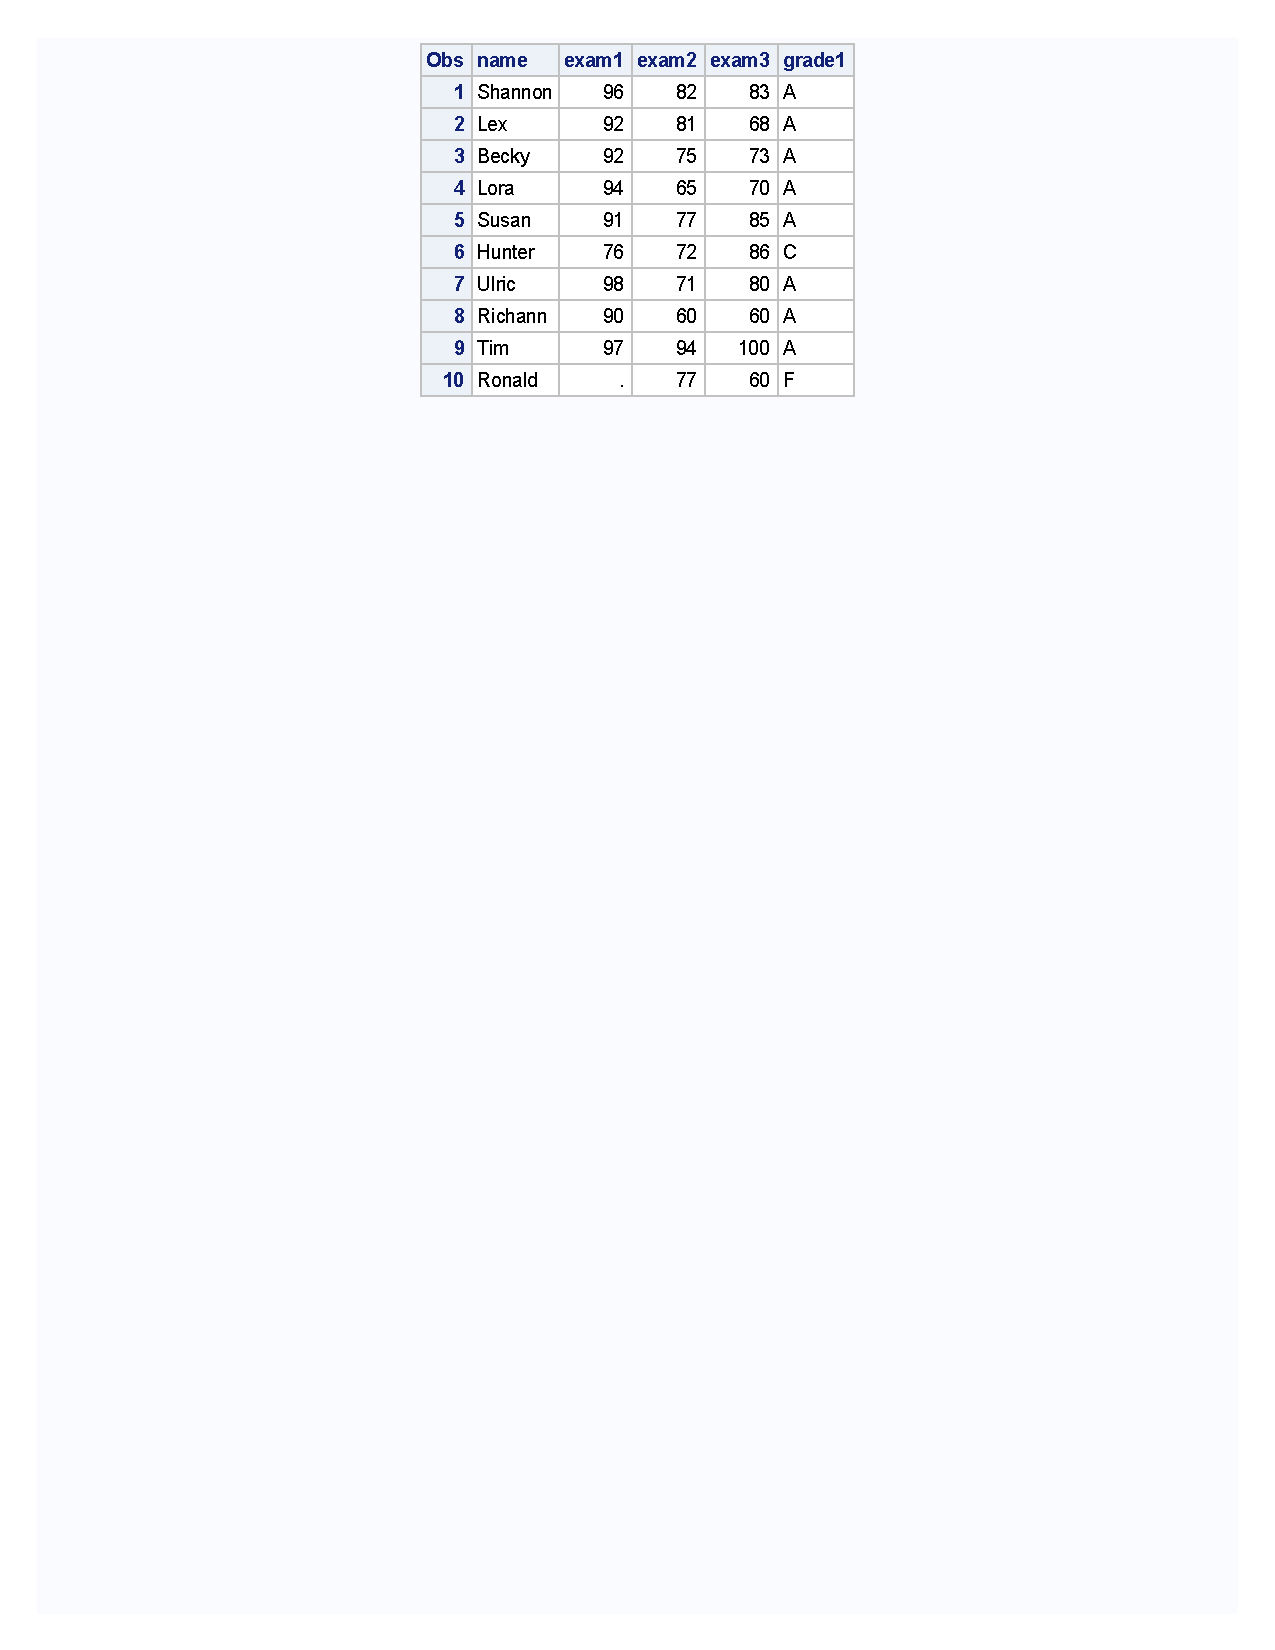
\includegraphics[trim={6cm 21cm 6cm 0.5cm},clip,width=1.0\textwidth]{L5_missingF.pdf}
\emp\\
\vskip10pt
\oyo Explain why Ronald's exam 1 grade is an F.  Propose a solution to fix it.
\end{frame}

%\begin{frame}[fragile]
%\ft{Missing values}
%When using the comparison operators, SAS treats missing observation values (.) as as the smallest possible value (e.g., negative infinity) .\\
%\vskip10pt
%\bmp{0.7\textwidth}
%\footnotesize
%\begin{code}{.0}
%data test1grade;
%    test1 = .;
%    if test1 >=  90 then grade1 = "A";
%    if 80 <= test1 < 90 then grade1 = "B";
%    if 70 <= test1 < 80 then grade1 = "C";
%    if 60 <= test1 < 70 then grade1 = "D";
%    if test1 < 60 then grade1 = "F";
%run;
%\end{code}
%\emp
%\bmp{0.1\textwidth} \hspace{0.1in} \emp
%\bmp{0.2\textwidth}
%\begin{clicker}{What is the value of \ttt{grade1}?}
%\begin{enumerate}
%    \item ``F''
%    \item `` ''
%    \item .
%    \item error
%\end{enumerate}
%\end{clicker}
%\emp
%\end{frame}



\begin{frame}[fragile]
\ft{IF/THEN/ELSE}
\bi
\item IF/THEN statements can be made more efficient by including an ELSE statement
\item When the IF \emph{condition} is met, the ELSE clause will be \ttb{ignored}
\item ELSE will carry out any actions only when the IF \emph{condition} is not met
\item SAS uses less computer time because once an observation satisfies the condition it can skip the rest of the IF / THEN series
\item This also ensures exclusive groups (ie. can’t meet two assumptions at once)
\ei
\bmp{1.0\textwidth}
\footnotesize
\begin{code}{.0}
IF \emph{condition} THEN action1;
ELSE action2;
\end{code}
\emp
\end{frame}

\begin{frame}[fragile]
\ft{Example Code IF/THEN/ELSE}
\bmp{0.8\textwidth}
\footnotesize
\begin{code}{.0}
DATA grades2;
   SET grades;
   IF exam1 >=  90 THEN grade1 = "A";
   ELSE IF 80 <= exam1 < 90 THEN grade1 = "B";
   ELSE IF 70 <= exam1 < 80 THEN grade1 = "C";
   ELSE IF 60 <= exam1 < 70 THEN grade1 = "D";
   ELSE IF 0  <= exam1 < 60 THEN grade1 = "F";
   ELSE grade1 = " ";
RUN;
\end{code}
\emp
\end{frame}

\begin{frame}[fragile]
\ft{IF/THEN for Multiple Actions}
\bi
\item Often, we want a computer program to take \ttb{several actions} if a specific condition is satisfied.
\item Use an IF/THEN with a DO/END statement to carry out this task
%\item Syntax: \ttt{IF \emph{condition} THEN DO \emph{action\myuscore 1}; \emph{action\myuscore 2}; ... \emph{action\myuscore k}; END;}
\item It is good programming practice to indent your code whenever you employ DO/END statements. It makes the code easier to read.
\ei
\bmp{1.0\textwidth}
\footnotesize
\begin{code}{.0}
IF \emph{condition} THEN DO;
    action1;
    action2;
END;
\end{code}
\emp
\end{frame}

\begin{frame}[fragile]
\ft{IF/THEN with Multiple Conditions}
\bi
\item Often, we want a computer program to take an \ttb{action} if a set  \ttb{conditions} are satisfied.
\item Use an IF/THEN with a AND/OR statement
\item Example: \ttt{IF \emph{condition\myuscore 1} AND \emph{condition\myuscore 2} THEN \emph{action};}
\item[]
\ei
\begin{tabular}{lll}
\hline
symbolic & mnemonic & notes \\
\hline\hline
\verb|&| & \ttt{and} & all comparisons must be true\\
\verb;|, !; & \ttt{or} & only one comparison needs to be true\\
 & \ttt{in}(\emph{list}) & similar to \ttt{or}\\
\hline
\end{tabular}
\end{frame}


\begin{frame}[fragile]
\ft{Example Code}
\hspace*{-0.35in}\bmp{0.80\textwidth}
\begin{code}{.0}
IF exam1 >=  90 THEN grade1 = "A";
ELSE IF 80 <= exam1 < 90 THEN grade1 = "B";
ELSE IF 70 <= exam1 < 80 THEN grade1 = "C";
ELSE IF 60 <= exam1 < 70 THEN grade1 = "D";
ELSE IF 0  <= exam1 < 60 THEN grade1 = "F";
ELSE grade1 = " ";
IF exam1 lt 80 and exam2 lt 80 THEN flag = "*  ";
ELSE flag = " " ;
IF grade1 in ("A", "B") THEN status = "honors";
ELSE status = "other" ;
IF exam1 = . and name = "Ronald" THEN DO;
   exam1 = 0 ;
   flag = "***" ;
END;
ave_exam = MEAN(exam1, exam2, exam3);
 \end{code}
\emp
\bmp{0.01\textwidth} \hspace{0.1in} \emp
\bmp{0.35\textwidth}
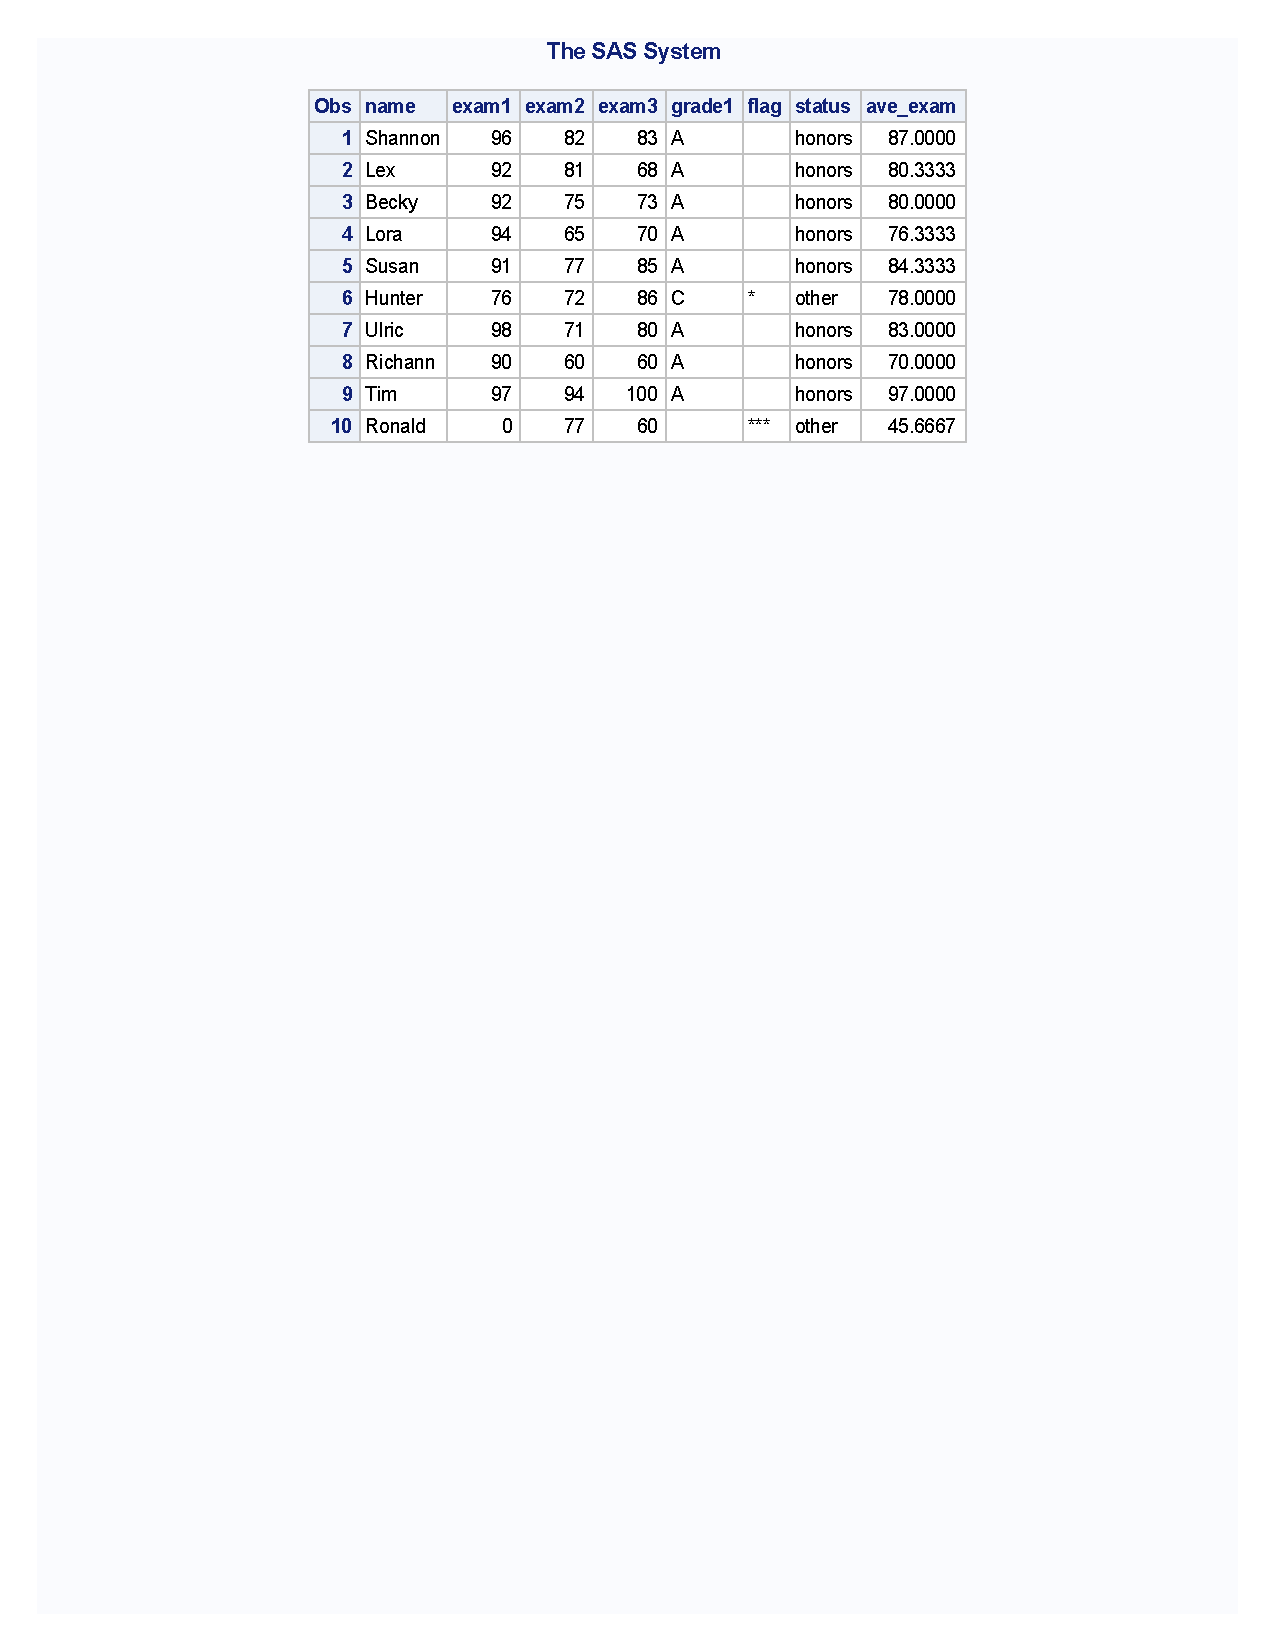
\includegraphics[trim={5cm 20cm 5cm 0.5cm},clip,width=1.0\textwidth]{L4_ite.pdf}
\emp\\
\end{frame}


\begin{frame}
\ft{Length of character variables}
\bi
\item When you create character variables, SAS determines the length of the variable from its \emph{first} occurrence in the DATA step.
\item Therefore, you must allow for the longest possible value in the \emph{first} statement that mentions the variable.
\item If you do not assign the longest value the first time the variable is assigned, then data can be truncated.
\item Two ways to fix this:
    \begin{enumerate}
        \item Assign the longest value first.
        \item Establish the length of the character variable in the data step \emph{before} you create the variable.
        \item[] \fbox{\ttt{LENGTH status \$ 6;}}
    \end{enumerate}
\ei
\end{frame}

%===========================================================================================================================
\section[DROP / KEEP variables]{DROP / KEEP variables}
%===========================================================================================================================
\subsection{}
\begin{frame}
\tableofcontents[currentsection, hideallsubsections]
\end{frame}
\begin{frame}
\frametitle{Drop/Keep}
\bi
\item Occasionally, it may be unnecessary or undesirable to keep all variables in a data set
\item To reduce the number of variables in your data set you can use \fbox{\ttt{DROP}} or \fbox{\ttt{KEEP}} statements
\item These can be used in two ways:
\begin{enumerate}
    \item As a statement in your DATA step
    \item As an option in your PROC
\end{enumerate}
\ei
\end{frame}



\begin{frame}[fragile]
\ft{Example Code - Method 1}
\bmp{0.7\textwidth}
\footnotesize
\begin{code}{.0}
DATA grades2 ;
   SET grades;
   ave_exam =  MEAN(exam1, exam2, exam3) ;
   DROP exam1 exam2 exam3;
RUN ;

PROC PRINT DATA = grades2 ;
RUN ;
\end{code}
\emp
\bmp{0.01\textwidth} \hspace{0.1in} \emp
\bmp{0.35\textwidth}
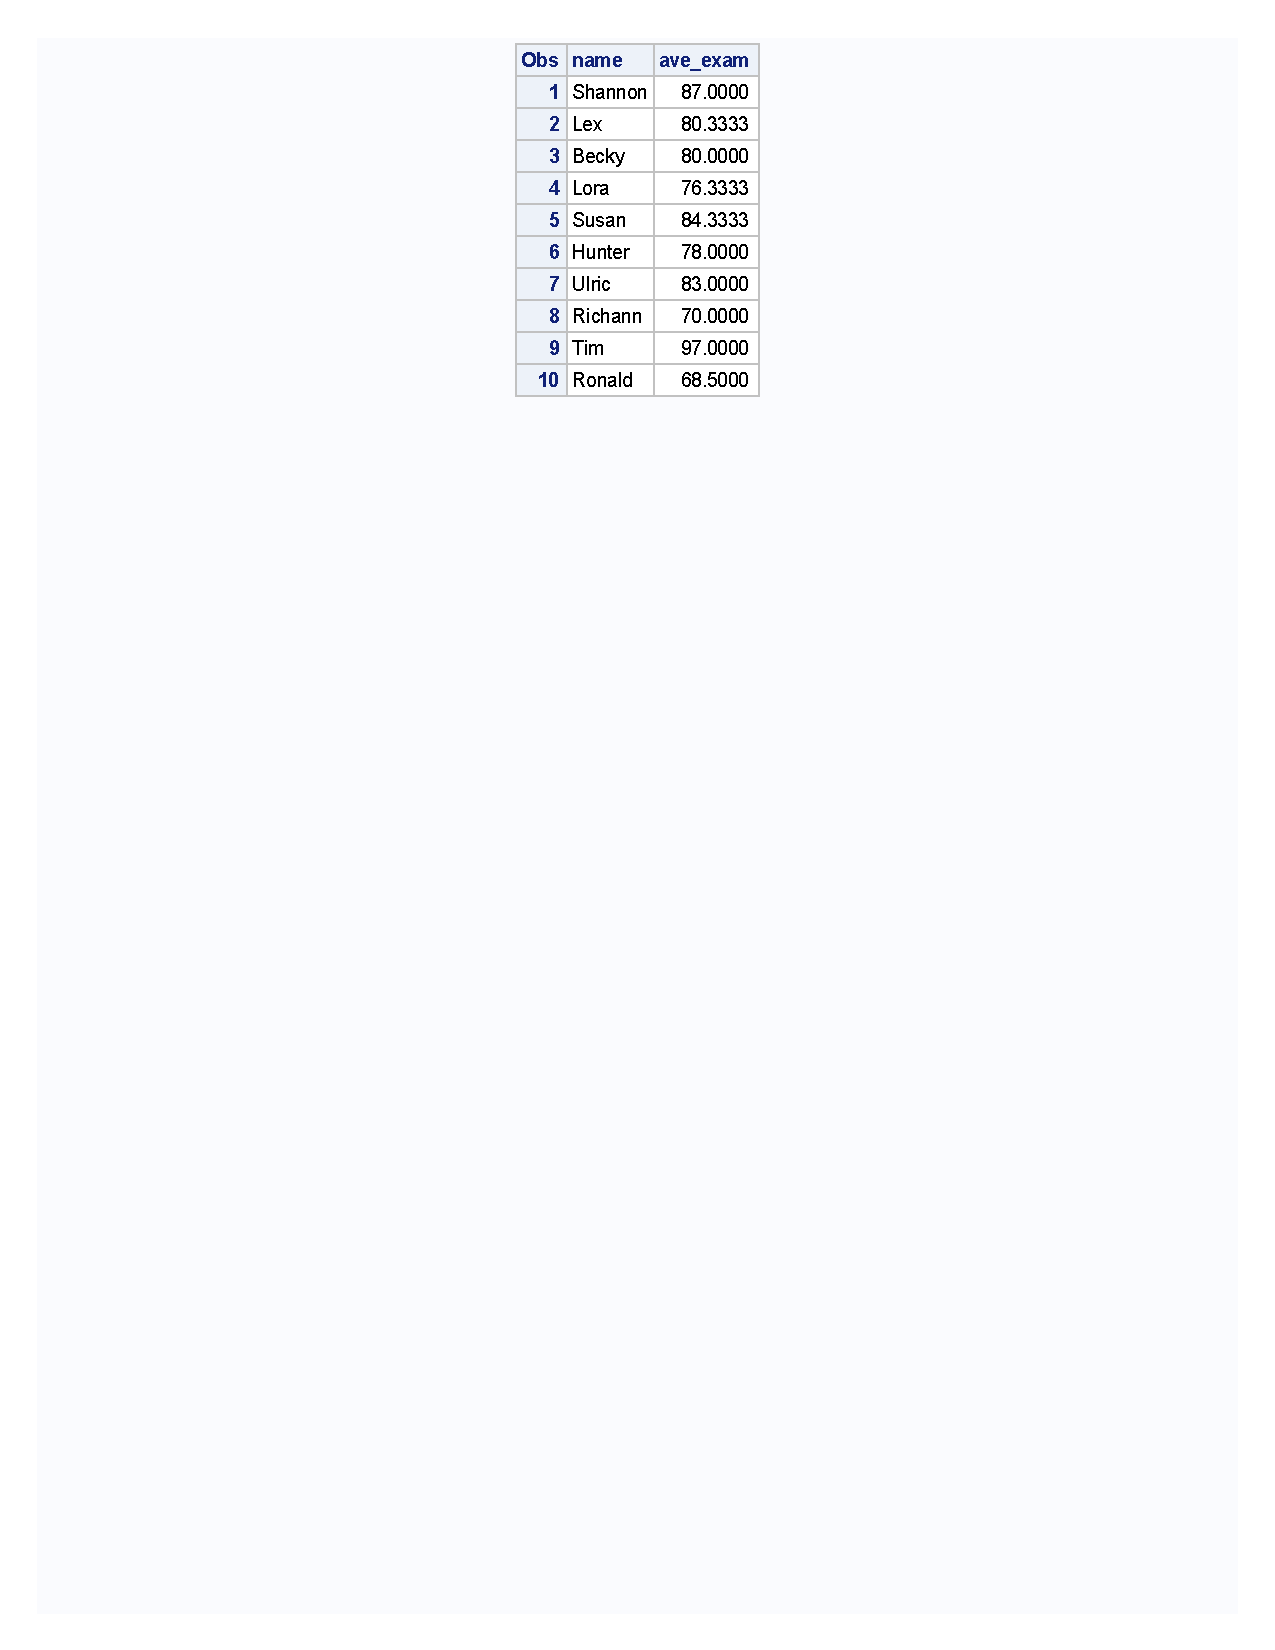
\includegraphics[trim={8cm 21cm 8cm 0.5cm},clip,width=1.0\textwidth]{L5_drop.pdf}
\emp\\
\vskip15pt
\oyo How could we re-state this using KEEP?
\end{frame}

\begin{frame}[fragile]
\ft{Example Code - Method 2}
\bmp{1.0\textwidth}
\footnotesize
\begin{code}{.0}
DATA grades2 ;
   SET grades;
   ave_exam =  MEAN(exam1, exam2, exam3) ;
RUN ;

PROC PRINT DATA = grades2 (DROP = exam1 exam2 exam3) ;
RUN ;
\end{code}
\emp
\end{frame}


%===========================================================================================================================
\section[Subsetting observations]{Subsetting observations}
%===========================================================================================================================
\subsection{}
\begin{frame}
\tableofcontents[currentsection, hideallsubsections]
\end{frame}

\begin{frame}
\ft{Overview of subsetting data}
Subsetting in DATA steps:
\begin{itemize}
\item can utilize both IF and WHERE to retain certain observations
\item[]
\end{itemize}

Subsetting in PROCs:
\begin{itemize}
\item can only utilize WHERE to perform procedures on certain observations in a data set
\end{itemize}
%\begin{tabular}{p{8cm} p{1cm} p{1cm} }
%Action & \ttb{\ttt{WHERE}} & \ttb{\ttt{IF}} \\
%\hline
%\ttt{DATA} - retain certain observations in a data set & \gc & \gc \\
%& & \\
%\ttt{PROC} - perform procedures on certain observations in a data set & \gc & \rx \\
%& & \\
%Can be use with raw data (e.g., a data step with an \ttt{infile} or \ttt{datalines} statement)   & \rx & \gc \\
%\hline
%\end{tabular}
\end{frame}

\begin{frame}[fragile]
\ft{Example code}
Retain only observations where exam 1 grade exceeds 90.\\
\vskip10pt
\hspace*{0.2in}
\bmp{0.6\textwidth}
\footnotesize
\begin{code}{.0}
DATA grades2 ;
   SET grades;
   IF exam1 > 90 ;
   /*EQUIVALENT STATEMENTS*/
   *IF exam1 > 90 THEN OUTPUT ;
   *IF exam1 <= 90 THEN DELETE ;
   *WHERE exam1 > 90 ;
RUN ;

PROC PRINT DATA = grades;
	WHERE exam1 > 90 ;
RUN;
\end{code}
\emp
\bmp{0.01\textwidth} \hspace{0.1in} \emp
\bmp{0.35\textwidth}
\includegraphics[trim={7cm 22cm 7cm 0cm},clip,width=1.0\textwidth]{L5_dataif.pdf}\\
\includegraphics[trim={7cm 22cm 7cm 0cm},clip,width=1.0\textwidth]{L5_procwhere.pdf}
\emp\\
\end{frame}

\begin{frame}[fragile]
\ft{More \ttt{WHERE} examples}
\bi
\item SAS's \ttt{WHERE} is modeled after the \ttt{where} in SQL programming.
\item Works similarly to \ttt{IF/THEN}, but is more efficient by avoiding unwanted observations
\item Can use additional \emph{operators}
\item[] \url{http://support.sas.com/documentation/cdl/en/lrdict/64316/HTML/default/viewer.htm#a000202951.htm}
\ei
\hspace*{0.2in}
\bmp{0.6\textwidth}
\footnotesize
\begin{code}{.0}
DATA grades2 ;
   SET grades;
   WHERE name contains "S" ;
RUN ;
\end{code}
\emp
\bmp{0.01\textwidth} \hspace{0.05in} \emp
\bmp{0.35\textwidth}
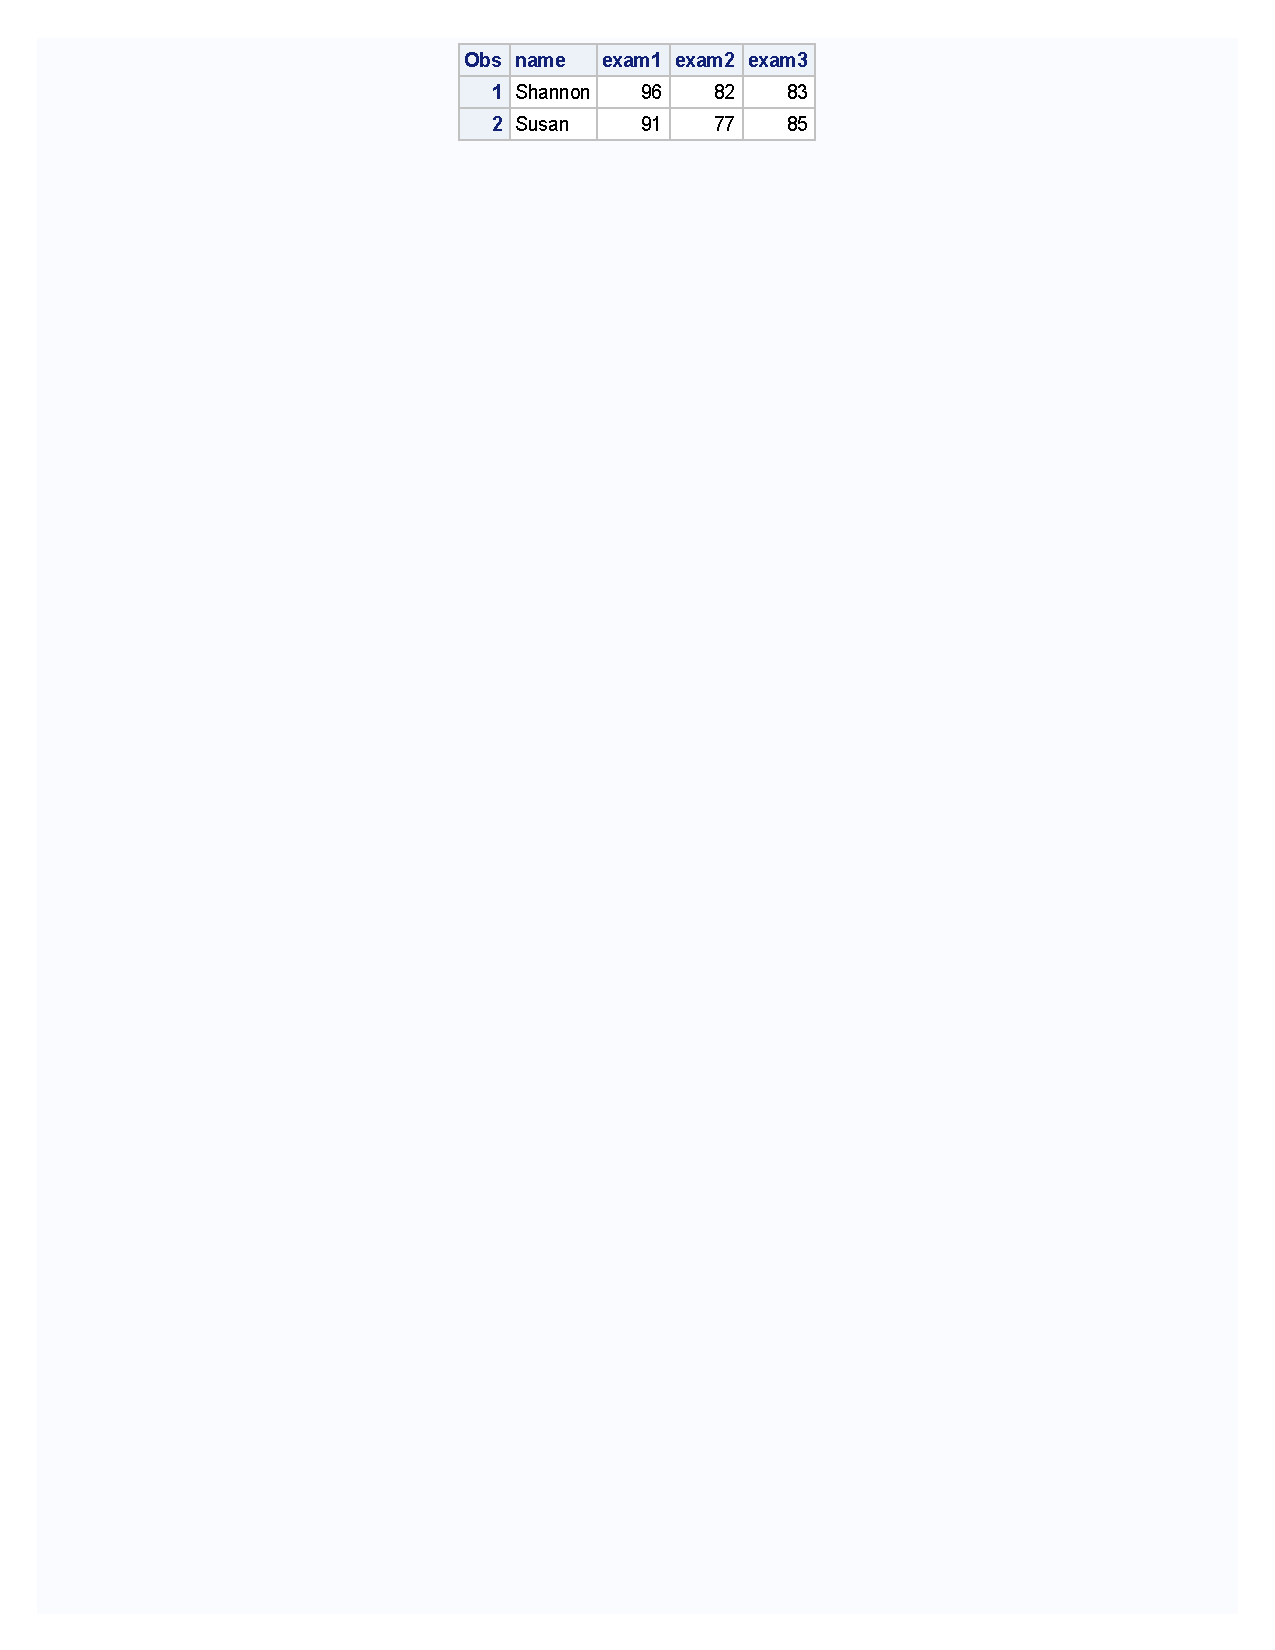
\includegraphics[trim={7cm 25cm 7cm 0cm},clip,width=1.0\textwidth]{L5_S.pdf}\emp
\end{frame}

\begin{frame}[fragile]
\ft{Subset to multiple data sets}
SAS can subset data into multiple data set within the \ttb{same} \ttt{DATA} step.
\hspace*{-0.2in}\bmp{0.70\textwidth}
\footnotesize
\begin{code}{.0}
DATA \textcolor{OrangeRed}{gradesA} \textcolor{OrangeRed}{gradesOther} ;
   SET grades ;
   IF exam1 >= 90 THEN OUTPUT \textcolor{OrangeRed}{gradesA} ;
   ELSE OUTPUT \textcolor{OrangeRed}{gradesOther} ;
RUN ;
\end{code}
\emp
\bmp{0.01\textwidth} \hspace{0.05in} \emp
\bmp{0.35\textwidth}
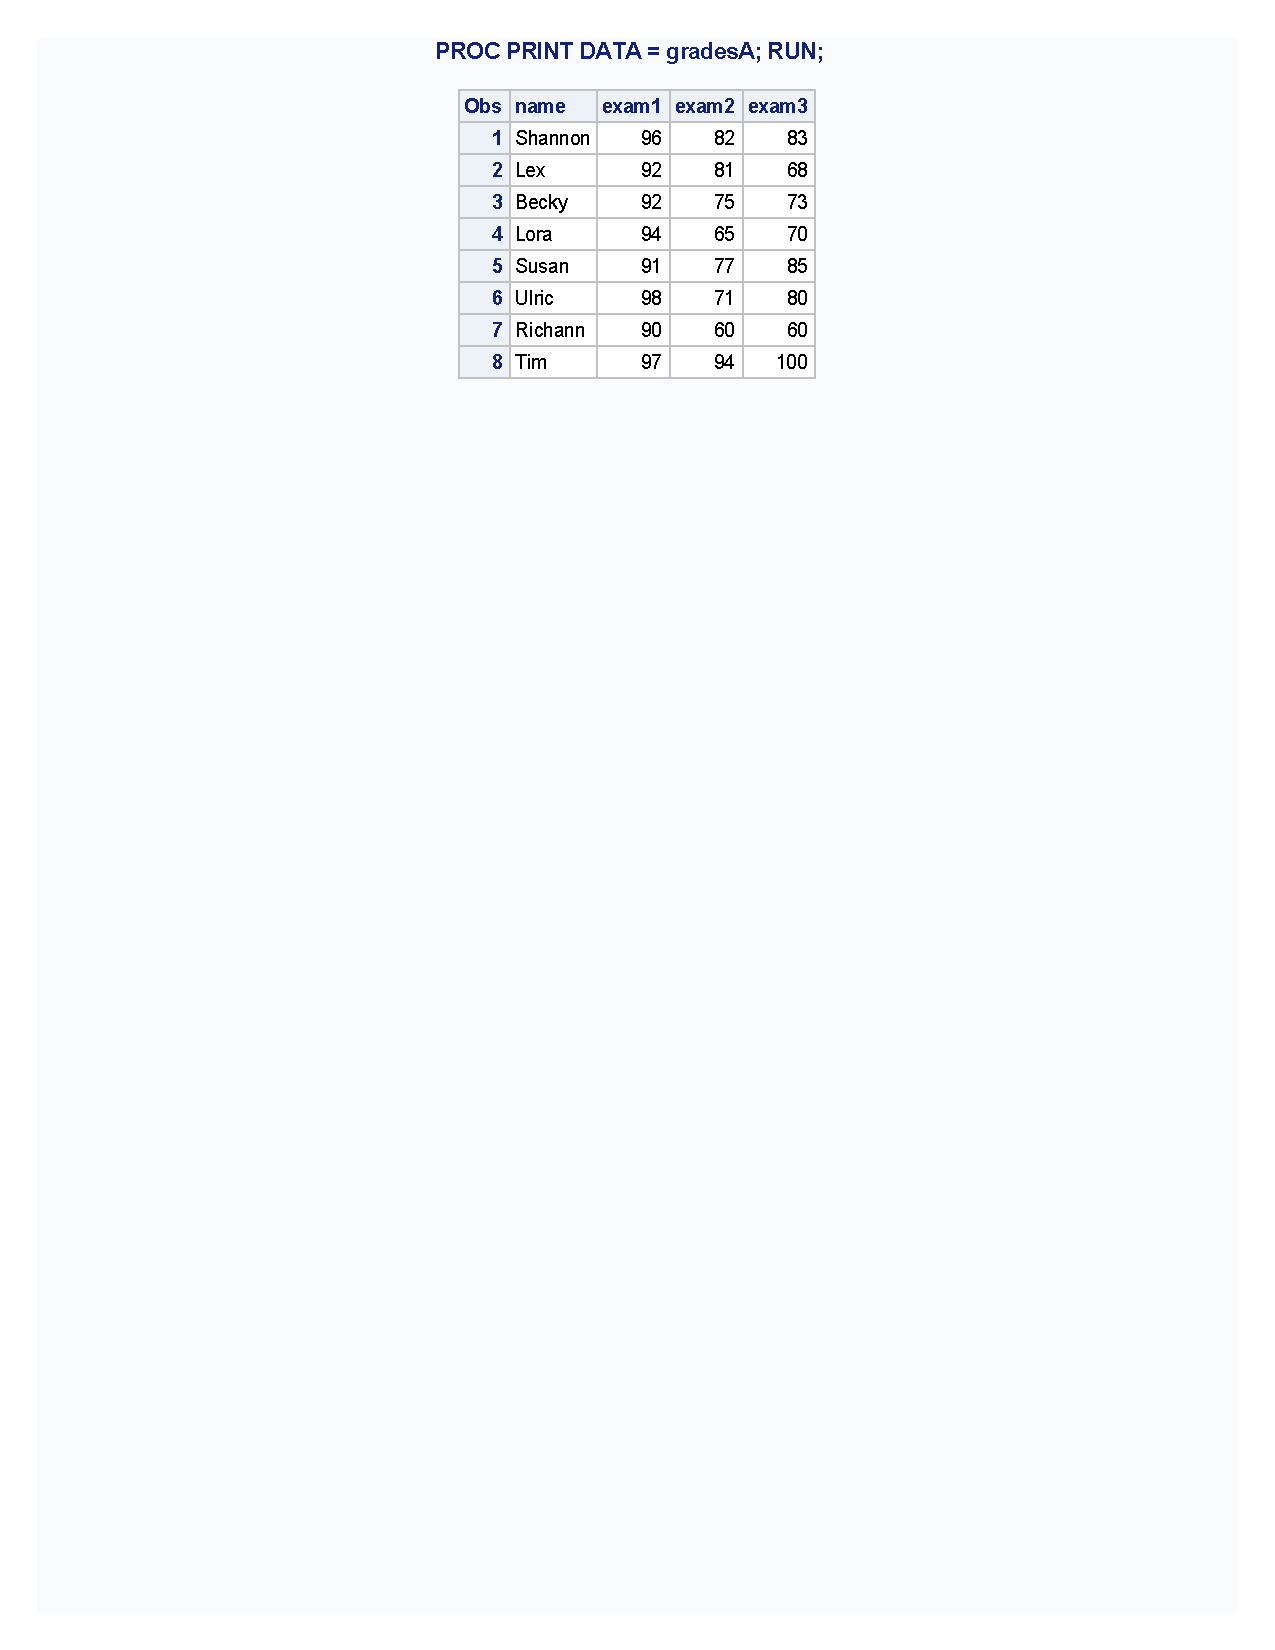
\includegraphics[trim={7cm 21cm 7cm 0cm},clip,width=1.0\textwidth]{L5_gradesA.pdf} \\
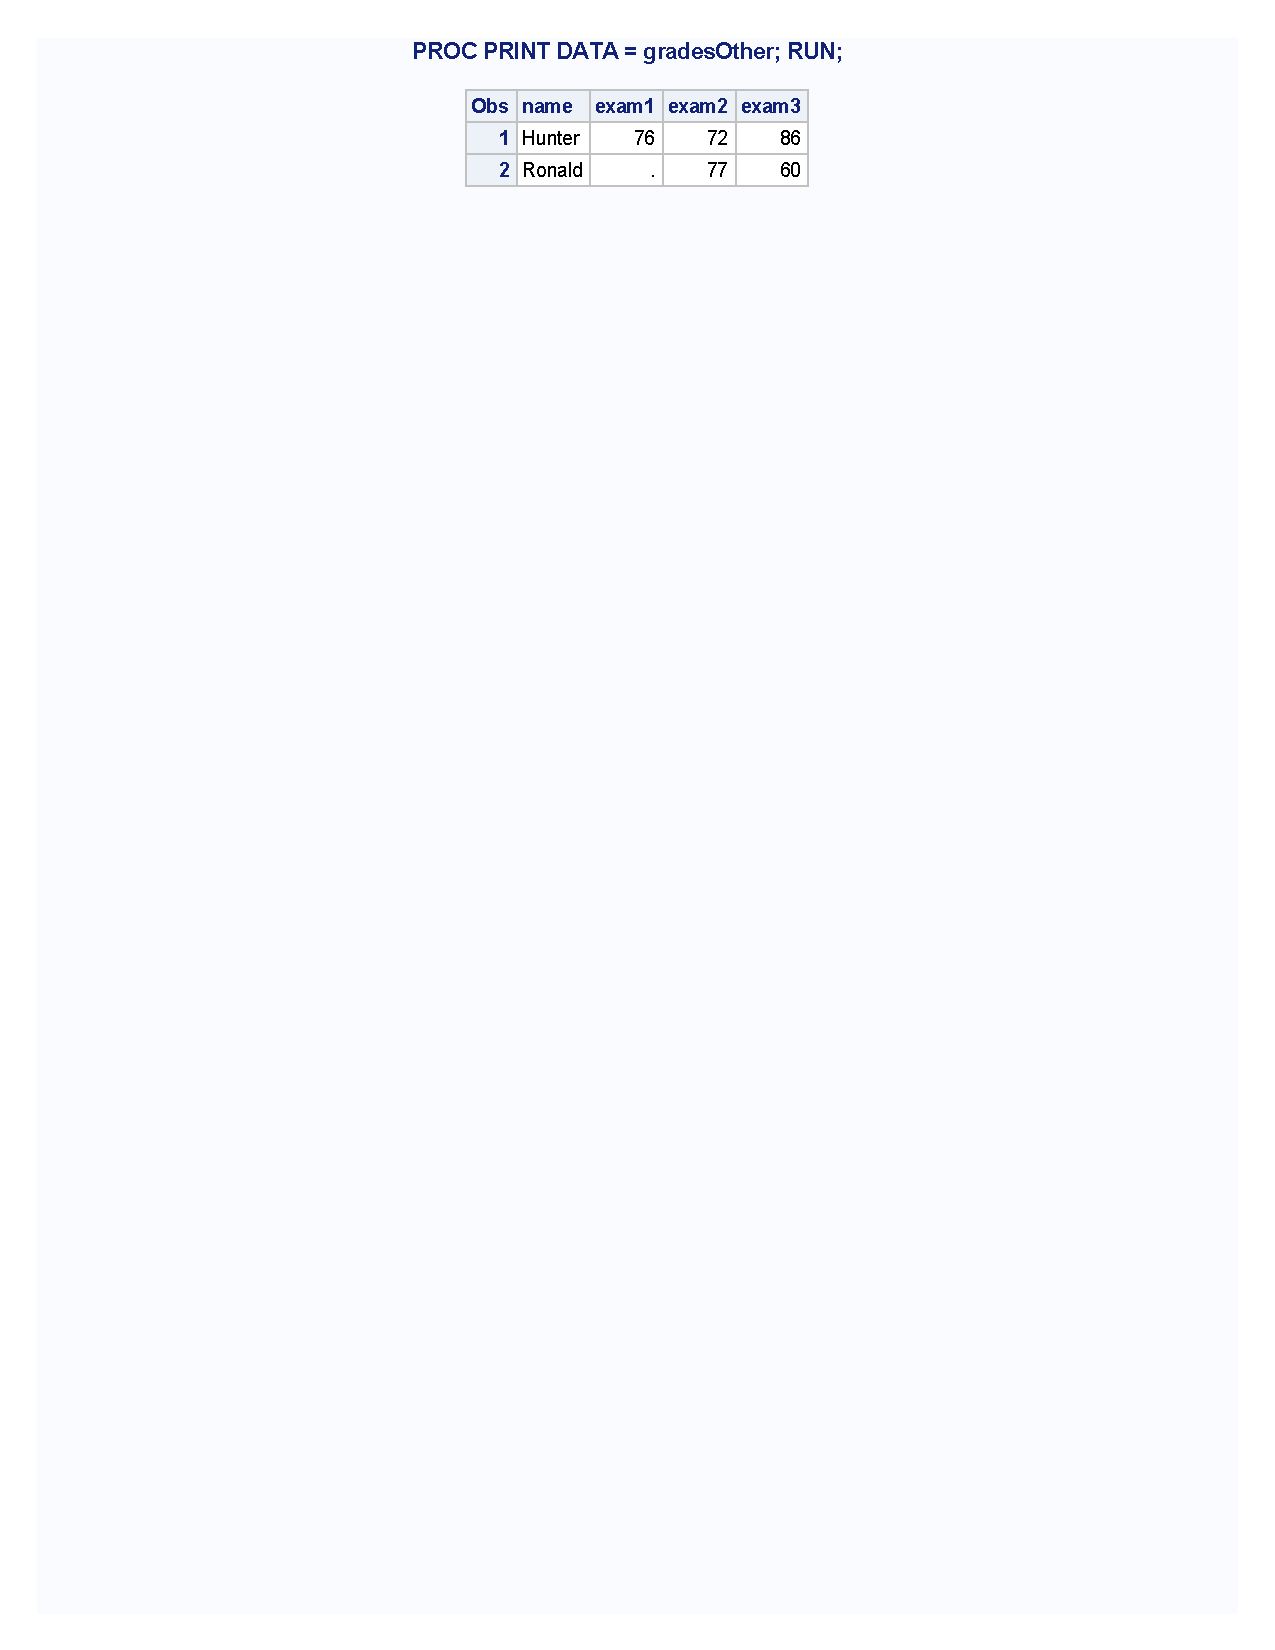
\includegraphics[trim={7cm 24cm 7cm 0cm},clip,width=1.0\textwidth]{L5_gradesOther.pdf}
\emp
\end{frame}

\end{document} 